\chapter{Generalized Bayesian Inference with Sets of Priors}

\begin{itemize}
\item Short introduction to IP (sets of priors, lower/upper prevision/probability)
%\item motivate imprecise priors with ress paper: \cite{Troffaes2013a} --- now in intro
\item \pdc\ (Evans \& Moshonov, Fuquene-Cook-Pericchi), examples (Festschrift paper: \cite{Walter2010a})
\item further motivations for IP (ITIP chapter \cite{itip-statinf}) 
\item Generalized Bayesian inference
\item Generalized Bayesian inference with sets of priors
 \begin{itemize}
 \item sets of priors, GBR, robust Bayes
 \item sets of conjugate priors in general
 \item parameter set shapes
 \end{itemize}
\item IDM
\item JSTP paper \cite{Walter2009a}
\item isipta11 paper \cite{Walter2011a}
\item boatshape?
\end{itemize}

Sec.~\ref{sec:imprecisebayes} is based on \textcite[\S 8.4.2]{itip-statinf}


After having seen a detailed example for Bayesian inference using sets of conjugate priors in Section~\ref{sec:commoncause},
in the main chapter of this thesis,
we will give now a general introduction to the methodology of Bayesian inference with sets of conjugate priors.
In Section ****, \\
Section **** 


\section{Imprecise or Interval Probability}
\label{sec:ip-intro}

This Section will give a condensed introduction to the main theoretic concepts
in interval or imprecise probability as needed for the topics discussed in this thesis.

While Section~\ref{sec:ip-general} follows mostly \textcite{2011:IESS-ip},
Section~\ref{sec:ip-main} is based mainly on \textcite{1996:walley::expert} and \textcite{2000:walley::towards}.


\subsection{General Concept and Basic Interpretation}
\label{sec:ip-general}

The central idea of imprecise or interval probability \parencite{2011:IESS-ip, 1991:walley, 2001:weichselberger} is
to replace the usual, precise probability measure $\p(A)$ for events $A$%
\footnote{Events of interest $A$ are taken to be subsets of the sample space $\Omega$,
forming a $\sigma$-algebra, a non-empty collection of sets including countable unions and intersections of subsets of $\Omega$.}
with a \emph{lower} and \emph{upper probability}, denoted by $\Pl(A)$ and $\Pu(A)$, respectively,
satisfying
\begin{equation}
\label{eq:0ip1}
0 \le \Pl(A) \le \Pu(A) \le 1\,.
\end{equation}
In this setting, a usual probability measure forms the extreme case $\Pl(A) = \Pu(A) = \p(A)$,
when there is enough information to determine the distribution on the sample space $\Omega$
in precise stochastic terms.
On the other extreme, when $\Pl(A) = 0$ and $\Pu(A) = 1$,
we have no information at all on the probability for $A$ to occur,
and intermediate cases $0 \le \Pl(A) < \Pu(A) \le 1$ represent
different degrees of knowledge on this probability.

Therefore, interval or imprecise probability adds another modeling dimension:
While usual, precise probability measures can be used to model phenomena when there is perfect stochastical information,
like, e.g., in a lottery where the number of winning tickets (and the total number of tickets) is precisely known,
imprecise probability measures can account for cases where there is uncertainty about the probabilities themselves,
just like in a lottery where the number of winning tickets is not exactly known.
Non-stochastic uncertainty about model features like probabilities is often called \emph{ambiguity},
forming a crucial part of the human decision process,
and there are studies suggesting that humans process ambiguity in a way
differing from pure probabilistic reasoning \parencite{2005:hsu-bhatt}.

In contrast to a probability measure $\p(A)$,
the set functions $\Pl(A)$ and $\Pu(A)$ do not adhere
to the additivity axiom of Kolmogorov's \parencite*{1933:kolmogorov}
formalization of probability as a normed measure,
%(countable or finite additivity),
and thus are also known as \emph{non-additive probabilities}.
There is also a link to \emph{fuzzy measures}, which are also non-additive measures
\parencite[see, e.g.,][]{1997:denneberg}.

In general, $\Pl(A)$ may be understood as accounting for evidence certainly in favour of $A$,
and $\Pu(A)$ accounting for all evidence speaking not strictly against $A$.
The difference of $\Pu(A)$ and $\Pl(A)$ thus allows for inconclusive evidence
that may not speak unanimously in favor of or against $A$, respectively.
As evidence strictly against $A$ can be seen as evidence certainly in favour of $A^\com$,
the complement of $A$,
it is mostly assumed that $\Pl(A^\com) = 1 - \Pu(A)$,
and thus it suffices to determine either of $\Pl$ or $\Pu$,
the other one being defined through this relation.

There are currently two main approaches to a general theory of statistical inference with interval or imprecise probability:
\begin{enumerate}[(i)]
\item The theory by \textcite{2000:weichselberger, 2001:weichselberger}
regards probability intervals $[\Pl(A), \Pu(A)]$ for all or some events $A$ as the basic entity
\parencite[p.~646]{2011:IESS-ip},
from which an interval-valued distribution on the sample space $\Omega$ is constructed.
His approach is axiomatic, in the sense that it replaces Kolmogorov's \parencite*{1933:kolmogorov} additivity axiom by two axioms,%
\footnote{The first states that \eqref{eq:0ip1} holds,
the second that the set $\mathcal{M}$ consisting of all usual, precise distributions $\p(\cdot)$
with $\Pl(A) \le \p(A) \le \Pu(A)$, for all $A \in \Omega$, is non-empty.
The second axiom guarantees that there exists at least one precise probability distribution
which is compatible with an interval-valued probability distribution,
and thus rules out the case of contradictory assignments of $[\Pl(A), \Pu(A)]$.}
from which the theory is derived,
while imposing no specific interpretation on these constructs.
This theory of interval probability was developed
as the foundation of a concept of \emph{logical probability} \parencite{2007:weichselberger},
where probability is not assigned to events, but to logical conclusions (from a premise to a consequence),
with the aim to arrive at a theory of statistical inference
which allows for fiducial-like probability statements,
e.g., probability statements on parameters similar to a posterior distribution in a Bayesian setting
without the need to specify a prior distribution \parencite{2011:IESS-fiducial}.
\item In contrast, the theory by Walley \parencite*{1991:walley, 2000:walley::towards}
aims to generalise the Bayesian approach to statistical inference,
adopting a strictly subjective, behavioural interpretation for imprecise probability
as lower and upper betting rates (see below),
and extending the Bayesian inference paradigm (as discussed in Section~\ref{sec:bayes-inference})
to imprecise probability distributions.
In generalising de Finetti \parencite*{1937:finetti,1970:finetti}, the basic entities are lower and upper \emph{previsions},
i.e.\ expectation functionals, for \emph{gambles}, i.e.\ random variables,
instead of lower and upper probabilities for events.
This is due to the fact that unlike in precise probability theory%
---where the definition of a distribution via expectations %precise previsions
(often denoted \emph{linear previsions} in the imprecise probability literature)
is eqivalent to a definition via a precise probability distribution---%
the definition of an imprecise distribution via lower and upper previsions
is more general than a definition via lower and upper probability for events
\parencite[p.~132]{2000:walley::towards}.
\end{enumerate}
As this thesis is concerned with a generalization of Bayesian inference
based on sets of conjugate priors, the approach by Walley,
and its reliance on a subjective, epistemic interpretation of (imprecise) probability
as (bounds for) betting rates, is now described in more detail.***


\subsection{Main Formulations}
\label{sec:ip-main}

%lower and upper probabilities or expectations,
%link to sets of probability distributions,
%sets of desirable gambles as mathematical formulation,
%lower and upper betting rates,
%inference procedure (itip)

The main mathematical formulations for imprecise distributions
in the theory by Walley \parencite*{1991:walley, 2000:walley::towards}
are
\begin{enumerate}[(i)]
\item lower previsions,
\item sets of (precise) probability distributions, and
\item sets of desirable gambles.
\end{enumerate}
It is possible to switch between these formulations,
although (ii) can be slightly more general than (i),
and to a greater extent, (iii) is more general than (ii) \parencite{2000:walley::towards}.

We will first introduce lower previsions
and the most important rationality requirements guiding their assessment and use,
then have a brief look at sets of desirable gambles as the most comprehensive formulation.
Sets of probability distributions, as the formulation used to describe inference models in this thesis,
are then explained in relation to the other formulations,
and the generalised Bayesian inference procedure as used in Section~\ref{sec:imprecise-alpha} is justified formally.

\paragraph{Lower Previsions}

As mentioned in Section~\ref{sec:ip-general}, the basic entities in the theory by \textcite{1991:walley}
are lower and upper \emph{previsions}.
These are functions on \emph{gambles}, or \emph{random variables},
defined as bounded mappings from $\Omega$ to $\reals$.
A gamble $X$ can be understood as uncertain reward or payout,
where the reward $X(\omega)$ depends on $\omega \in \Omega$,
the unknown `state of the world' from the possibility space $\Omega$.
The reward is measured in units of utility assumed to form a linear scale
\parencite[\S 2.2]{1991:walley}.

A \emph{lower prevision} or \emph{lower expectation} is then a mapping
$\El: \mathcal{K} \to \reals$, where $\mathcal{K}$ is a set of \emph{gambles}.%
\footnote{In Walley's central monography \parencite{1991:walley},
his papers and the imprecise probability literature in general,
lower previsions are usually denoted by $\Pl$.
There, an event $A \subset \Omega$ is notationally identified with the
indicator function $I_A(\omega)$, being a gamble with payout $1$ if $\omega \in A$ and else $0$,
such that $\Pl(A)$ denotes the lower probability of $A$.
In order to follow conventions in statistical literature, however,
lower previsions are denoted by $\El$ here,
and $\Pl$ refers to lower probabilities only.}
Central to Walley's theory is the interpretation of $\El[X]$
as the subject's supremum buying price for $X$, that is,
the subject is disposed to pay at most the fixed amount $\El[X]$
in exchange for the uncertain reward $X$.%
\footnote{More precisely, the price the subject is disposed to pay for $X$ is strictly less than $\El[X]$.
For sake of readability,
this mathematically important distinction is not rigorously maintained in this brief overview,
as it is hardly relevant for the interpretation of the results in the later parts of this thesis.}
$\El[X]$ thus expresses the subject's state of knowledge about the value of $X$,
factoring in the propensity of all possible $\omega \in \Omega$
with their specific payouts $X(\omega)$.
The \emph{upper prevision} $\Eu[X]$ is the infimum selling price for $X$,
i.e., the fixed amount the subject is willing to receive in exchange for $X$
\parencite[p.~9]{1996:walley::expert}.
Walley's theory is based on this behavioral, epistemic interpretation of previsions,
%\parencite[Section~4]{1996:walley::expert},
and all rationality criteria and inference procedures
are deduced from this root \parencite[p.~5]{1996:walley::expert}.

The theory allows thus a zone of indeterminacy, by $\El[X] < \Eu[X]$,
for prices of $X$ at which the subject is neither willing to buy or to sell the gamble $X$,
as illustrated in Figure~\ref{fig:pricesforgambles}.
This is in contrast to the usual epistemic operationalisation of subjective Bayesian probability,
which implies that $\El[X]$ and $\Eu[X]$ must coincide at a unique fair price $\E[X]$.
This requirement is refuted by Walley, and called by him \emph{the Bayesian dogma of (ideal) precision}
\parencite[\S 5]{1991:walley}.

\begin{figure}
\centering
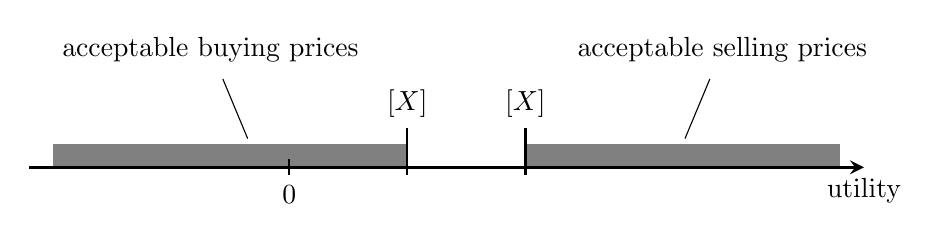
\begin{tikzpicture}[%
linkline/.style={
  shorten >= 2pt,
  shorten <= 3pt
}%
]
\path[fill=gray] (0,0) rectangle (4.5,0.3);
\path[fill=gray] (6,0) rectangle (10,0.3);
\draw[very thick,-stealth] (-0.3,0) -- (10.3,0) node[below] {utility};
\draw[thick] (3,0.1) -- (3,-0.1) node[below] {$0$};
\draw[thick] (4.5,-0.1) -- (4.5,0.5) node[above] {$\El[X]$};
\draw[thick] (6,-0.1) -- (6,0.5) node[above] {$\Eu[X]$};
\node (buy) at (2,1.5) {acceptable buying prices};
\node (sell) at (8.5,1.5) {acceptable selling prices};
\draw[linkline] (buy) -- (2.5,0.3);
\draw[linkline] (sell) -- (8,0.3);
\end{tikzpicture}
\caption{\label{fig:pricesforgambles}%
Illustration of \underline{E}\ and $\Eu$ as supremum buying and infimum selling prices for a gamble $X$ on a linear utility scale.}
%$\El$ %strange errors occur
\end{figure}

A lower and upper prevision are called \emph{conjugate}%
\footnote{Conjugacy in this sense should not be confused
with conjugacy for prior distributions as discussed in Section~\ref{sec:regularconjugates}.}
if the relation $\Eu[X] = -\El[-X]$ holds for all $X \in \mathcal{K}$.%
\footnote{This implies the relation $\Pl(A^\com) = 1 - \Pu(A)$
of lower and upper probabilities for events $A \subset \Omega$
as mentioned in Section~\ref{sec:ip-general}.}
Then, it suffices to consider only either of $\El$ or $\Eu$,
and in the literature $\El$ is chosen,
the theory consequently being referred to as the theory of
\emph{coherent lower previsions} \parencite[See, e.g.,][\S 3.2]{itip}.

\paragraph{Coherence and Avoiding Sure Loss}

Before we come to the concept of \emph{coherence},
a weaker rationality requirement put forward by Walley is
that a lower prevision $\El$ should fulfill the property of
\emph{avoiding sure loss} \parencite[\S 2.4]{1991:walley}.
This means that a subject, whose state of information about the
occurence of `states of the world' from the possibility space $\Omega$
is encoded in his or her choice of $\El$,
acting by buying and selling gambles accordingly,
should choose $\El$ such that there is no combination of gambles
%$X_i$, $i=1,\ldots,k$, %of which each is, by $\El$, 
that would result in a net loss, whatever $\omega \in \Omega$.
As an analogy, \emph{avoiding sure loss} can be regarded
like a logical inconsistency in a set of propositions,
i.e., there exist two propositions in the set of propositions
(the analogy to $\El$) which are contradictory
\parencite[\S 2.4, footnote~1]{1991:walley}.

Continuing this analogy, $\El$ violating the stronger property of \emph{coherence}
is like the ``failure to deduce all [\ldots] logical implications''
\parencite[\S 2.4, footnote~1]{1991:walley} from the set of propositions.
As an example, if a subject assesses $\El$ such that $\El[X] = \El[Y] = \frac{1}{4}$,
and also that $\El[X+Y] = \frac{1}{4}$, $\El$ avoids sure loss, but is not coherent,
because one can imply from $\El[X] = \El[Y] = \frac{1}{4}$ that
$\El[X+Y]$ must be at least $\frac{1}{2}$ \parencite[p.~67]{1991:walley}.
Coherence is a ``normative requirement of consistency'' \parencite[p.~130]{2000:walley::towards}
that is a consequence of few basic rationality requirements.
In fact, if $\mathcal{K}$ is a linear space of gambles,
i.e., $\mathcal{K}$ is closed with respect to addition and multiplication with constants,
then coherence is equivalent to the three following conditions
\parencite[e.g.,][p.~11]{1996:walley::expert}:
\begin{enumerate}[(i)]
\item $\El[X] \ge \inf_{\omega \in \Omega} X(\omega)$,
i.e., one is always prepared to buy a gamble for less than its minimum possible reward.
(Being prepared to pay more than $\inf_{\omega \in \Omega} X(\omega)$ amounts to make a commitment to the
possibility that other states $\omega'$ with $X(\omega') > \inf_{\omega \in \Omega} X(\omega)$ may occur.)
\item $\El[\lambda X] = \lambda \El[X]$ for all $X \in \mathcal{K}$, $\lambda > 0$.
$\El$ should be such that if it postulates that one should be prepared to buy a gamble $X$ at a price
of at most $\El[X]$, then one should also buy gambles that are fractions or multiples of $X$
at prices of at most the original price divided or multiplied accordingly.
This illustrates that prices are to be understood on a linear utility scale
(as mentioned above) and should not be considered as plain monetary prices,
for which this condition may not be reasonable.
\item $\El[X+Y] \ge \El[X] + \El[Y]$.
This property of superlinearity implies that the supremum acceptable buying price for $X$ and $Y$ combined
should be at least the sum of supremum acceptable buying prices for each of $X$ and $Y$ individually.
It could be, e.g., that $X$ and $Y$ balance out each other in a way that
buying both of them at once makes the transaction less risky,
such that a higher price limit for $X + Y$ is acceptable.
Usual precise expectations, for which additivity $\E[X+Y] = \E[X] + \E[Y]$ must hold,
cannot directly accommodate such reasoning.
\end{enumerate}

Consequently, in analogy to deducing all logical implications from
a set of propositions, there is a technique, %for lower previsions,
called \emph{natural extension}, that adjusts
a given assessment of lower and upper previsions (on some set of gambles $\mathcal{K}$, which must avoid sure loss)
to make it coherent, in the least committal way as possible%
\footnote{This means that there may be other adjustments of $\El$ that are compatible
with the initial assessments, but are less conservative,
i.e., give higher supremum buying prices.}
\parencite[see, e.g.,][pp.~15ff]{1996:walley::expert}.
This is accomplished by a linear program,
and may involve raising $\El[X]$ for some $X \in \mathcal{K}$ in order to make them
coherent to the values of $\El[Y]$, supremum buying prices for some other gambles $Y \in \mathcal{K}$ as previously assessed,
or newly defining $\El[Z]$ for gambles $Z$ not considered during assessment---explaining the name `extension'.

\paragraph{Sets of Desirable Gambles}

Sets of desirable gambles \parencite[\S 6]{2000:walley::towards} are an alternative formulation
for probability assessments as expressed by a lower prevision $\El$.
They are a mathematically convenient formulation
and as such a central and very useful tool in the development of the theory of imprecise probability.
However, a detailed understanding of this concept is not necessary for the purpose of this thesis,
and the account below is inteded to complete the overview on the theory of imprecise probability.

The \emph{gambles} here are again a description of an uncertain reward as above, 
and all bounded functions from $\Omega$ to $\reals$
are forming the space $\mathcal{L}$ of all gambles.
The assessment in this formulation lies in the designation of a subset $\mathcal{D}$
of all gambles $\mathcal{L}$ as \emph{desirable gambles},
i.e., as supplying an uncertain reward (in utilities) for which,
from the subject's state of information
about the propensity of occurence of the different $\omega \in \Omega$,
the potential benefits outweigh the potential losses.
Thus, all gambles $X$ that will never incur a loss,
$\{X: X \ge 0\}$, where $X \ge 0$ denotes that $X(\omega) \ge 0\ \forall \omega \in \Omega$,
should be contained in a coherent set of desirable gambles $\mathcal{D}$.
Indeed, the notion of \emph{coherence} for lower previsions translates to sets of desirable gambles as follows:
$\mathcal{D} \subset \mathcal{L}$ is coherent if and only if
\parencite[p.~137]{2000:walley::towards}
\begin{enumerate}[(D1)]
\item $0 \notin \mathcal{D}$ ($0$ is the gamble $X$ with $X(\omega) = 0\ \forall \omega \in \Omega$),
\item if $X \in \mathcal{L}$ and $X > 0$ then $X \in \mathcal{D}$\\
($X > 0$ denotes that $X \ge 0$ and $\exists \omega \in \Omega: X(\omega) > 0$),
\item if $X \in \mathcal{D}$ and $c \in \posreals$ then $cX \in \mathcal{D}$,
\item if $X \in \mathcal{D}$ and $Y \in \mathcal{D}$ then $X+Y \in \mathcal{D}$.
\end{enumerate}
In $\mathcal{L}$, a coherent set of gambles $\mathcal{D}$ is thus a convex cone
containing all positive gambles $\{X: X > 0\}$ but not the zero gamble.%
\footnote{As the weaker property, a set of gambles $\mathcal{D}$ avoids sure loss
if $\posi(\mathcal{D}) \cap \{X: X(\omega) < 0\ \forall \omega \in \Omega\} = \emptyset$.
Here, $\posi(\mathcal{D}) := \{ \sum_{i=1}^n c_i X_i : c_i \in \posreals, X_i \in \mathcal{D}, n \in \naturals \}$
is the positive hull of $\mathcal{D}$, 
i.e.\ the set of gambles resulting from application of (D3) and (D4) on $\mathcal{D}$.}

A coherent set of desirable gambles can be derived from a coherent lower prevision $\El$ by
\parencite[p.~139]{2000:walley::towards}
\begin{align*}
\mathcal{D} = \left\{ X \in \mathcal{L} :
X > \sum_{i=1}^n c_i (X_i - \El[X_i] + \epsilon) \text{ for some } n \in \naturals, c_i > 0, \epsilon > 0, X_i \in \mathcal{L} \right\}\,.
\end{align*}
If we adopt $\El$ as the lower prevision expressing our beliefs about $\Omega$,
gambles $X_i - \El[X_i] + \epsilon$ should be desirabe for us;
considering the price $\El[X_i]$ as the supremum acceptable buying price for $X_i$,
the gamble $X_i - \El[X_i]$ should---in our view---be at least as good as the zero gamble.

Conversely, a coherent lower prevision can be deduced from a coherent set of desirable gambles by
$\El[X] := \sup\{c: X - c \in \mathcal{D}\}$.
%\parencite[p.~139]{2000:walley::towards}
If we make $c$ as large as possible such that the gamble $X-c$ is still acceptable to us,
then $\El[X]$ simply is our supremum acceptable buying price for $X$.

As already mentioned, sets of desirable gambles are a more general formulation
as compared to lower previsions, illustrated by the fact that there can be
several sets $\mathcal{D}$ leading to the same $\El$ \parencite[p.~139]{2000:walley::towards}.%
\footnote{Another formulation equivalent to sets of desirable gambles is the description as \emph{partial preference orderings},
where a partial ordering of the gambles in $\mathcal{L}$ is given to express beliefs on $\Omega$
\parencite[p.~138]{2000:walley::towards}.}

\paragraph{Sets of Probability Distributions}

We now turn to the formulation of imprecise probability assessments
applied in this thesis, 
sets of (precise) probability distributions,
which are also called \emph{credal sets} \parencite[p.~136]{2000:walley::towards}.

There is a one-to-one correspondence between lower coherent previsions
and non-empty, closed and convex sets of (precise) probability distributions
\parencite[\S 3.6.1]{1991:walley}.
When dropping the conditions of convexity and closure,
sets of probability distributions can be slightly more general
than coherent lower previsions \parencite[\S 5]{2000:walley::towards}.
However, the nature of this slight increase in generality is not relevant here,
although we will consider the question of convexity more closely later.

Given a coherent lower prevision $\El$,
the corresponding set of distributions $\mathcal{M}$
is closed and convex, and consists of all probability distributions
whose expectations $\E_p$ dominate $\El$, i.e.,
\begin{align*}
\mathcal{M} &= \{ p(\omega) : \E_p[X] \ge \El[X]\ \forall X \in \mathcal{L}\}\,.
\end{align*}
In fact, for all $p \in \mathcal{M}$ and $X \in \mathcal{L}$,
the relation $\El[X] \le \E_p[X] \le \Eu[X]$ holds;
the set $\mathcal{M}$ consists of all probability distributions
whose expectations are compatible with the bounds defined by
the lower prevision $\El$ and its conjugate upper prevision $\Eu$.

Conversely, given a non-empty set of probability distributions $\mathcal{M}$,
where $\mathcal{M}$ needs not necessarily be closed or convex,
the corresponding coherent lower prevision, for any gamble $X \in \mathcal{L}$,
is defined by
\begin{align*}
\El[X] &= \inf_{p \in \mathcal{M}} \E_p[X]\,,
\end{align*}
and in this case, $\El$ is called the \emph{lower envelope} of $\E_p$, $p \in \mathcal{M}$
\parencite[p.~132]{1991:walley}.

There are very important relations between the notions of avoiding sure loss and coherence on the one hand,
and the formulation of imprecise probability assessments via sets of probability distributions on the other hand.
The two equivalences below are known as the \emph{lower envelope theorem} \parencite[\S 3.3.3]{1991:walley}.
\begin{enumerate}[(a)]
\item $\El$ avoids sure loss if and only if the corresponding set $\mathcal{M}$ is non-empty.
Thus, an assessment $\El$ for which there is no compatible probability distribution
must incur a sure loss, and cannot be considered as reasonable.
On the contrary, any imprecise probability distribution defined by assigning
a set $\mathcal{M}$ of probability distributions avoids sure loss.
\item Furthermore, $\El$ is coherent if and only if it can be
described as the lower envelope based on its corresponding $\mathcal{M}$.
Therefore, all coherent lower previsions are characterised as
lower envelopes based on some set of precise distributions $\mathcal{M}$,
and imprecise probability assignments established via a such set $\mathcal{M}$
are coherent.
\end{enumerate}

Although the one-to-one correspondence mentioned above holds only for closed and convex sets $\mathcal{M}$,
there is nothing in the theory preventing us to consider
open or non-convex sets $\mathcal{M}$ as our probability model, %the initial assessment,
because lower and upper previsions derived from $\mathcal{M}$ are nevertheless coherent.

%link to lower previsions, convexity
%
%lower envelope theorem: itip Prop.~3.7, p.~58, 1991:walley Prop.~3.3.3
%
%itip sec.3.2.2, 3.3.3

\paragraph{Conditioning and the Generalised Bayes' Rule}

To use imprecise probability distributions for statistical inference
in the same way as usual Bayesian inference employs precise probability distributions,
we need a notion of \emph{conditioning} or \emph{updating} for imprecise probability distributions.
In analogy to the procedure described in Section~\ref{sec:bayes-inference},
the objective is to express prior knowledge on a parameter of interest $\vartheta$
by an imprecise prior distribution,
and all inferences shall be based on a (imprecise) posterior distribution derived from it.
As in Bayesian inference with precise distributions,
the now imprecise prior should be conditioned on the observed data $\x$.

A coherent lower prevision can be conditioned on an event $B$
by using the so-called \emph{Generalised Bayes' Rule} \parencite[\S 6.4]{1991:walley},
by which the conditioned coherent lower prevision $\El[X\mid B]$
based on a lower prevision $\El[X]$ can be derived.
$\El[X\mid B]$ is then also coherent to $\El[X]$, i.e.,
it is a model satisfying the rationality criteria as discussed for $\El[X]$
now also for the beliefs expressed in $\El[X]$ contingent on $B$.

In the formulation via a credal set, the Generalised Bayes' Rule
is equivalent to conditioning each distribution in the credal set on $B$
\parencite[\S 6.4.2]{1991:walley},
and the set of conditioned distributions is thus an equivalent model for $\El[X\mid B]$.
This result is known as the \emph{lower envelope theorem for conditional previsions}.

%GBR: coherence of prior and posterior

\subsection{Imprecise Bayesian Inference Procedure}
\label{sec:imprecisebayes}

%paragraph from itip

Walley has thus established a general framework for coherent statistical inference under imprecise probabilities.
It allows to transfer the basic aspects of traditional Bayesian inference to the generalized setting,
as the fundamental paradigms of Bayesian inference as discussed in Section~\ref{sec:bayes-inference} are maintained.
Prior knowledge on the parameter, expressed by a now imprecise prior distribution $\Pi(\cdot)$ with credal set $\mathcal{M}$,
is updated in the light of the observed sample $\x$ to the posterior $\Pi(\cdot \mid \x)$,
with the credal set $\mathcal{M}_{\vert \x}$,
and this statistical inference is again understood as a deductive process,
obtained directly by conditioning on the observed sample,
now according to the Generalized Bayes' Rule that ensures coherence of this inferential process.
For practical implementation of the Generalized Bayes' Rule, the lower envelope theorem for conditional 
previsions mentioned above %\parencite[\S~6.4.2]{1991:walley}
is of particular relevance.
The prior credal set $\mathcal{M}$ is updated element by element to obtain the posterior credal set %$\mathcal{M}_{\vert \mbf{x}}$
\begin{align*}
\mathcal{M}_{\vert \mbf{x}} = \left\{ p(\cdot \mid \x) :  p(\cdot) \in \mathcal{M} \right\}\,,
\end{align*}
consisting of all posterior distributions obtained
by traditional Bayesian updating of elements of the prior credal set.

Walley's lower envelope theorem also establishes a close connection to robust Bayesian approaches and Bayesian sensitivity analysis
(see, e.g.\ \parencite{2000:rios, 2005:ruggeri}) based on sets of distributions.
The basic difference is in the interpretation of the underlying sets of probability distributions.
While in the imprecise probability context a credal set is understood as an entity of its own,
the robust Bayesian approach emphasizes the single elements in the set,
and very often discusses the effects of deviations from a certain central element.
%As a consequence, for the robust Bayesian point of view it is quite natural and common
%to impose some further regularity conditions on the elements in the set of distributions,
%like additional smoothness constraints or unimodality of the underlying densities.
%Since lower and upper posterior probabilities are determined by the extreme points of the underlying credal sets, this distinction may indeed matter substantially in practice.
%\bigskip
Robust Bayesian inference and Bayesian sensitivity analysis
understand robustness and insensitivity mostly as desirable properties,
while the imprecise probability framework may use such behavior actively in modelling,
in particular in the context of prior-data conflict (see Section~\ref{sec:imprecisebayes-conjugate})***.


\subsection{Related Concepts}

many links to concepts that aim to complement probability theory as tool for handling uncertainty,
like possibilistic reasoning, fuzzy probabilities, etc.




\section{***Motivations for IP}

Although strictly negated by advocates of Bayesian methods \parencite[e.g., by][]{1987:lindley},
the need to go beyond usual probability measures has been recognized for a long time,%
\footnote{\textcite{2009:hampel} and \textcite[\S 1]{2001:weichselberger} give a historical overview on the development of
ideas related to non-additive measures and interval probability.}
and in recent times most prominently by scientists involved in the development of expert systems \parencite{1996:walley::expert}.

***klir citation (festschrift)***

\subsection{\pdc }

\subsection{Weakly Informative Priors}


\subsection{Other Motives}


\section{Generalised Bayesian Inference for Sets of Conjugate Priors in Exponential Families}
\label{sec:imprecisebayes-conjugate}

section itip / JSTP paper



%for later in IDM/IBBM discussion:\\
%we use Walley's \cite[\S 7.7.3, p.~395]{1991:walley} $(s,\vec{t})$ notation for the hyperparameters.
